\documentclass{article}
\usepackage[utf8]{inputenc}
\usepackage{graphicx}		% Graphics.
\usepackage{color}
\usepackage[english]{babel}
\usepackage{float}
\usepackage{subcaption}
\usepackage{xfrac}
\usepackage{amsmath}
\usepackage{amssymb}
\usepackage{siunitx}
\usepackage{titlesec}
\usepackage{enumitem}
\usepackage{longtable}
\usepackage[justification=centering]{caption}
\usepackage{adjustbox}
\usepackage[version=4]{mhchem}
\usepackage{expl3}
\usepackage{physics}
\usepackage{longtable}
\usepackage{matlab-prettifier}

% Create a separate table for the appendix.
\usepackage[toc,page]{appendix}

% Table of Content has fast links to sections.
\usepackage{hyperref}

% Remove dots in table of contents.
\usepackage[titles]{tocloft}
\renewcommand{\cftdot}{}

% Page style.
\usepackage[top=2cm, bottom=2cm, left = 2cm, right = 2cm]{geometry}
\setlength{\parindent}{0pt}	% Disable indents.

% BIBLATEX, BIBER as bibtex
\usepackage[style=ieee]{biblatex}
\usepackage{csquotes}
\addbibresource{references.bib}

% Get more layers for the sections.
\setcounter{secnumdepth}{4}
\titleformat{\paragraph}
{\normalfont\normalsize\bfseries}{\theparagraph}{1em}{}
\titlespacing*{\paragraph}
{0pt}{3.25ex plus 1ex minus .2ex}{1.5ex plus .2ex}


\begin{document}

%----------------------------------------------------------------------------------------
%	TITLE PAGE.
%----------------------------------------------------------------------------------------
%----------------------------------------------------------------------------------------
%	TITLE PAGE.
%----------------------------------------------------------------------------------------

\begin{titlepage} % Suppresses displaying the page number on the title page and the subsequent page counts as page 1.
	\center % Centre everything on the page.
	\newcommand{\HRule}{\rule{\linewidth}{0.5mm}} % Defines a new command for horizontal lines, change thickness here.
	
	
	%------------------------------------------------
	%	Logo.
	%------------------------------------------------
	\includegraphics[width=0.4\textwidth, trim=0 0 0 -2cm]{figures/LTU_logo.jpg}\\[1cm]
		
	
	%------------------------------------------------
	%	Headings.
	%------------------------------------------------
	\textsc{\Huge Lule\aa \ University of Technology}\\[1.5cm]
	
	\textsc{\LARGE Spacecraft Environment Interactions}\\[0.3cm]
	
	\textsc{\large R7004R}\\[0.5cm]
	
	
	%------------------------------------------------
	%	Title.
	%------------------------------------------------
	\HRule\\[0.4cm]
	
	{\Huge\bfseries Spacecraft Environment Interaction with a Hyperbolic Orbit}\\[0.4cm]
	
	\HRule\\[1.5cm]
	
	
	%------------------------------------------------
	%	Authors & supervisor.
	%------------------------------------------------
	\begin{minipage}{0.4\textwidth}
		\begin{flushleft}
			\large
			\textit{Authors:}\\
			D. Talavera\\
			E.F.M. Weterings
		\end{flushleft}
	\end{minipage}
	~
	\begin{minipage}{0.4\textwidth}
		\begin{flushright}
			\large
			\textit{Supervisors}\\
			J. Ejemalm\\
		\end{flushright}
	\end{minipage}
	
	
	%------------------------------------------------
	%	Date.
	%------------------------------------------------
	\vfill\vfill\vfill % Position the date 3/4 down the remaining page.
	
	{\large\today} % Date, change the \today to a set date if you want to be precise.
	
	
\end{titlepage}


%----------------------------------------------------------------------------------------
%	SUMMARY (-).
%----------------------------------------------------------------------------------------
\newpage				% Start at new page.
\thispagestyle{empty}	% Remove page numbering.
\phantomsection
\addcontentsline{toc}{section}{Abstract}
%----------------------------------------------------------------------------------------
%	SUMMARY.
%----------------------------------------------------------------------------------------
\section*{\label{sec:abstract}Abstract}


%----------------------------------------------------------------------------------------
%	TABLE OF CONTENT.
%----------------------------------------------------------------------------------------
\newpage				% Start at new page.
%\pagenumbering{arabic}	% Page numbering reset & style.
\renewcommand{\contentsname}{Table of Contents}
\tableofcontents		% Add table of content.


%----------------------------------------------------------------------------------------
%	INTRODUCTION (DIEGO).
%----------------------------------------------------------------------------------------
\newpage
%----------------------------------------------------------------------------------------
%	INTRODUCTION.
%----------------------------------------------------------------------------------------

\section{\label{sec:intro}Introduction}

The purpose of this report is to analyze the space environment of the trajectory followed to the fictional satellite Willzyx I. This in order to comply with a preliminary design review and determine if the proposed design is suitable to operate in the environment that exists in the surroundings of the planned trajectory. The radiation interaction and its interactions with certain components of the spacecraft will be analyzed using SPENVIS.

\subsection{Mission Definition}

The trajectory of Willzyx 1 is hyperbolic, with its closes approach to earth at 629\,km and a low inclination of only \ang{10}. A hyperbolic trajectory means that the satellite is traveling faster than the escape velocity of the planet or moon is passing by. Such trajectories are used for the so called "flybys" of satellites on celestial bodies, and can be used in order to do measurements of the celestial body they are passing by. This is common in order to perform observations or calibrations while en route to the final destination of the spacecraft, usually during gravitational assists.

\subsection{Orbitography}

\begin{figure}[H]
\centering
\includegraphics[scale=1]{figures/OrbitParameters.png}
\caption{Parameters of Willzyx I trajectory}
\label{OrbitParam}
\end{figure} 

In figure \ref{OrbitParam} above we can see the parameters of the trajectory followed by Willzyx I. These are the parameters used in order to numerically simulate and plot the orbit. 

\begin{figure}[H]
\centering
\includegraphics[width=0.68\textwidth]{figures/Trajectory.png}
\caption{Trajectory of the spacecraft during 1 day}
\label{Trajectory}
\end{figure}  

Inf figure \ref{Trajectory} the trajectory of the spacecraft around the Earth is shown. As mentioned before, since this is a hyperbolic trajectory (and therefore not a closed orbit), it will escape Earth after the flyby.

\begin{figure}[H]
\centering
\includegraphics[width=0.78\textwidth]{figures/GroundTrack.png}
\caption{Ground Track of the spacecraft during the flyby}
\label{GroundTrack}
\end{figure}

Figure \ref{GroundTrack} shows the path that Willzyx I will have on the surface of the Earth during the flyby. Due to it's low inclination it will stay very close to the Equator.



%----------------------------------------------------------------------------------------
%	GENERAL DESCRIPTION OF SPACECRAFT ENVIRONMENT (DIEGO).
%----------------------------------------------------------------------------------------
\newpage
%----------------------------------------------------------------------------------------
%	GENERAL.
%----------------------------------------------------------------------------------------

\section{\label{sec:general}General Spacecraft Environment Description}



%----------------------------------------------------------------------------------------
%	NUMERICAL SIMULATIONS (DIEGO & ELRICK).
%----------------------------------------------------------------------------------------
\newpage
%----------------------------------------------------------------------------------------
%	NUMERICAL SIMULATIONS.
%----------------------------------------------------------------------------------------

\section{\label{sec:simulations}Numerical Simulations}

%----------------------------------------------------------------------------------------
%	LIFE TIME & PERFORMANCE DEGRADATION (DIEGO).
%----------------------------------------------------------------------------------------
\subsection{\label{subsec:life}Life Time \& Performance Degradation}


%----------------------------------------------------------------------------------------
%	TOTAL DOSE & SHIELDING (DIEGO).
%----------------------------------------------------------------------------------------
\subsection{\label{subsec:shield}Total Dose \& Shielding}


%----------------------------------------------------------------------------------------
%	SINGLE EVENT UPSETS (Elrick).
%----------------------------------------------------------------------------------------
\subsection{\label{subsec:SEU}Single Event Upsets}
A single event upset (or bit flip) happens when radiations strikes the electronics on the PCB of the spacecraft. It can then ionize a couple of atoms in a (field effective) transistor which can cause a current to flow. This current causes the so called single event effects, of which the most common one is called a single event upset (SEU). This happens when the current is low enough to not burn the components (then it would be a single event burnout) but high enough to flip a bit in a memory device and thus corrupt the data stored. In order to have less SEU the memory should be shielded and/ or a redundancy computer can be implemented that compares memory. In the latter case the data should be stored on different memory devices using a RAID (Redundant Array of Independent Disks) protocol.\\

In table \ref{tab:SEU} the most important parameters for the TTL and CMOS chips are shown. It can be seen that the CMOS chip is larger, uses less energy but has a longer delay. The most important parameter for the SEU is the noise margin. This is for the CMOS chip higher than for the TTL chip. This means that a larger offset for a single bit must be given before the data is corrupted. In applications where power and data protection is key, the CMOS chip is a better solution. This is for instance the case in spacecrafts.

\begin{center}
\begin{longtable}{|p{4cm}|p{6.1cm}|p{6.1cm}|}

\hline \multicolumn{1}{|c|}{\textbf{}} & \multicolumn{1}{c|}{\textbf{TTL}} & \multicolumn{1}{c|}{\textbf{CMOS}} \\ \hline 
\endfirsthead

\multicolumn{3}{c}%
{{\bfseries \tablename\ \thetable{} -- continued from previous page}} \\
\hline \multicolumn{1}{|c|}{\textbf{}} & \multicolumn{1}{c|}{\textbf{TTL}} & \multicolumn{1}{c|}{\textbf{CMOS}} \\ \hline 
\endhead

\hline \multicolumn{3}{|r|}{{Continued on next page}} \\ \hline
\endfoot

\hline \hline
\endlastfoot

Method: & bipolar junction transistors (BJTs) & field effect transistors (FETs) ie.,by connecting NMOS and PMOS (MOSFETs) \\\hline

Gates used: & NAND & NAND-NOR \\\hline

Power consumption: & $\approx$10\,mW & $\approx$10\,nW \\\hline

Delay: & $\approx$10\,ns & $\approx$70\,ns \\\hline

Noise Margin: & $\approx$0.5\,V & $\approx$1.5\,V \\\hline

Data density: & higher & lower \\\hline

\caption{Comperisment TTL and CMOS chips \cite{TTL-CMOS}.}
 \label{tab:SEU}
\end{longtable}
\end{center}


%----------------------------------------------------------------------------------------
%	LET-SPECTRUM (Elrick).
%----------------------------------------------------------------------------------------
\subsection{\label{subsec:let}Linear Energy Transfer (LET) Spectrum}
To estimate the SEU rate, firstly the LET spectrum has to be estimated. Using SPENVIS the plot in figure \ref{fig:LET-shielding} has been made. Here it has been taken into account that there is an effective shielding of 1\,g/cm$^2$. If aluminum is used with a density of 2.7\,g/cm$^3$, then the shielding thickness is 0.37\,cm. 

\begin{figure}[H]
\centering
\includegraphics[width=.9\textwidth]{figures/LET-shielding.png}
\caption{Differential and Integrated flux of ions from hydrogen to uranium, as a function of the linear energy transfer (LET), with an effective shielding of 1\,g/cm$^2$, shielding tickness of 0.37\,cm with aluminium. The volume is 38.7\,x\,38.7\,x\,2\,$\mu$m \cite{SPENVIS}.}
\label{fig:LET-shielding}
\end{figure}

The integral representation of the SEU rate $\dv{U}{t}$ is given by equation \ref{eq:LET}. Here $\sigma$ is the experimentally determined cross section of a device as a function of LET and angles $(\theta,\phi)$. $h$(LET) is the differential fluxes of ions as functions of LET, summed over all relevant ion species (also called the LET spectrum).

\begin{equation}
\dv{U}{t} = \int^{2 \pi}_0 \int^\pi_0 \sin{\theta} \int^{\infty}_0 \sigma(\text{LET}, \theta, \phi) \cdot \sum^{92}_{Z=1} h(\text{LET}) d(\text{LET}) \,d\theta\,d\phi \label{eq:LET}
\end{equation}

The first two integrals in equation \ref{eq:LET} can be simplified to $4 \pi$. Thus the equation can be simplified to equation \ref{eq:LET2}.
\begin{equation}
\dv{U}{t} = 4 \pi \int^{\infty}_0 \sigma(\text{LET}, \theta, \phi) \cdot \sum^{92}_{Z=1} h(\text{LET}) d(\text{LET})\label{eq:LET2}
\end{equation}

The size chosen is 38.7\,x\,38.7\,x\,2\,$\mu$m. This means that, in the worst case scenario without taking into account the spacecraft charging ($\phi$), the cross section $\sigma$ is 1.5\,nm$^2$. However, for this example the cross section is ignored $\sigma = 1$. The differential flux summed over the elements H (hydrogen) to U (uranium) $\sum^{92}_{Z=1} h(\text{LET})$ is given as the straight line in figure \ref{fig:LET-shielding}.\\

When integrating over the differential flux and multiplying this result by 4$\pi$, as done in the MATLAB program in appendix \ref{app:matlab:LET}, the figure \ref{fig:matlab:LET-shielding} is obtained. Here the blue and red line are the original data, obtained from SPENVIS. The yellow line is the integrated flux by hand over the differential flux from SPENVIS. It can be seen that it doesn't quite match the integral flux from SPENVIS. This can be explained that SPENVIS re-calculates it's integral data to get a better precision. This means that it takes more data into account for bigger values of LET, which it does not provide to the user. This explains the difference on the right hand side. The difference on the left hand side can be explained by a difference method to determine the effectiveness of the shielding. Shielding mostly blocks the particles with a lower amount of energy.

\begin{figure}[H]
\centering
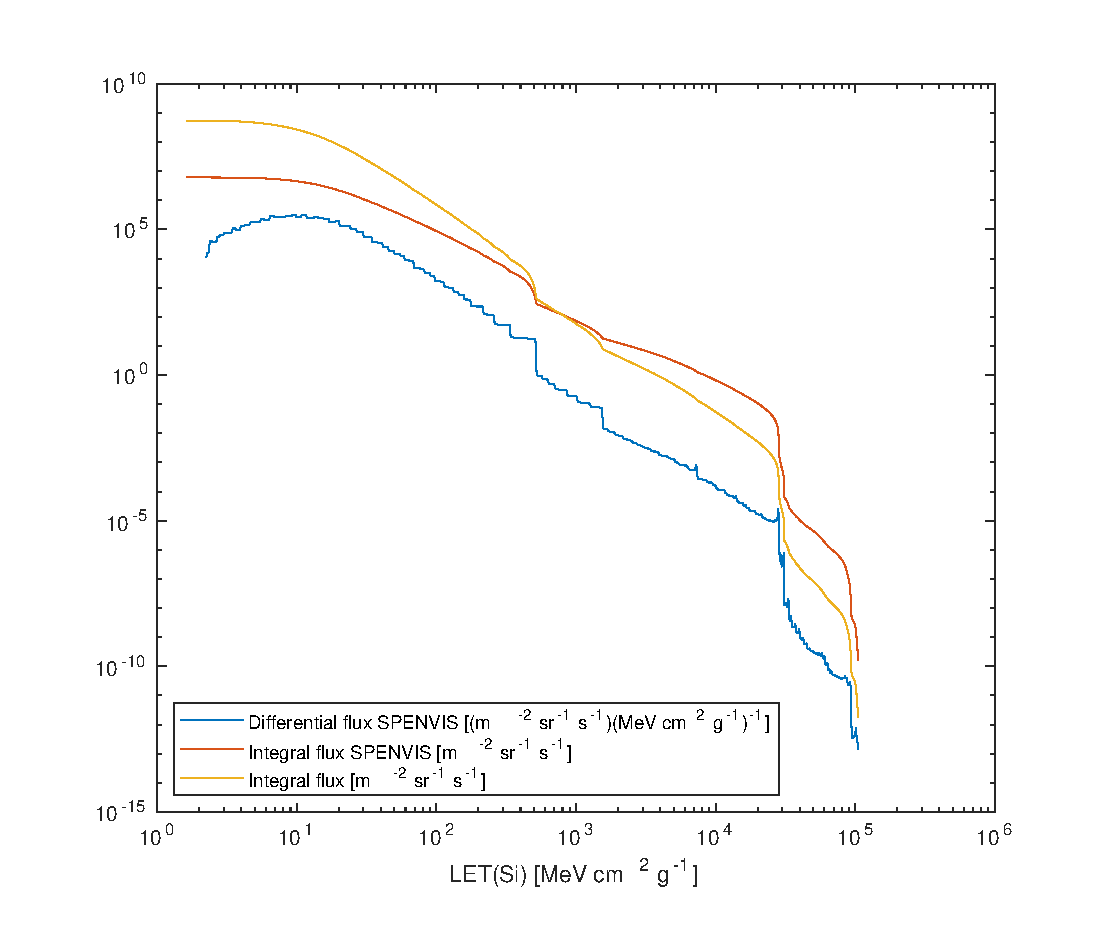
\includegraphics[width=.7\textwidth]{data/LET/LET.eps}
\caption{The differential flux (blue) and integral flux (red) obtained from SPENVIS and the integral flux (yellow) calculated with the MATLAB program in appendix \ref{app:matlab:LET}.}
\label{fig:matlab:LET-shielding}
\end{figure}


%----------------------------------------------------------------------------------------
%	CROSS SECTION \& COMPONENTS CHARACTERISTICS (Elrick).
%----------------------------------------------------------------------------------------
\subsection{\label{subsec:CSCC}Cross Section and Components Characteristics}
For some components the  characteristics are known are given. For this mission the SMJ329C50GFAM66 chip is used, this chip only has direct measurements available, as shown in table \ref{tab:SMJ-LET}. To find the cross section and the sensitivity of this chip, a Weibull function has to be fitted to the this data.

\begin{table}[H]
\centering
\begin{tabular}{|l|l|l|l|l|}
\hline
Ion & Energy Beam & Flux particles & Exposure time & Flips \\
& [MeV] & [cm$^{-2}$s$^{-1}$] & [minutes] & \\\hline

$^{12}$C & 0.60 & $25 \cdot 10^6$ & 5 & 8\\\hline
$^{12}$C & 0.72 & $25 \cdot 10^6$ & 5 & 7497\\\hline
$^{12}$C & 9.6 & $25 \cdot 10^6$ & 5 & 22514\\\hline
$^{16}$O & 4.8 & $17 \cdot 10^6$ & 5 & 23986\\\hline
$^{40}$Ar & 20 & $23 \cdot 10^6$ & 5 & 33810\\\hline
$^{56}$Fe & 56 & $10 \cdot 10^6$ & 10 & 29991\\\hline
$^{84}$Kr & 84 & $7 \cdot 10^6$ & 10 & 21022\\\hline
$^{131}$Xe & 786 & $4 \cdot 10^6$ & 15 & 18043\\\hline

\end{tabular}
\caption{SMJ329C50GFAM66 chip measurements}
\label{tab:SMJ-LET}
\end{table}

Dividing the energy of the beam in table \ref{tab:SMJ-LET} with the ion number the LET stopping power can be read from figure \ref{fig:LET-stoppingpower}.

\begin{figure}[H]
\centering
\includegraphics[width=1\textwidth]{figures/stoppingPower.png}
\caption{CREME Stopping Powers in Silicon.}
\label{fig:LET-stoppingpower}
\end{figure}

The cross section ($\sigma$) in cm$^2$ can be calculated from equation \ref{eq:sigma}. Here the N is the number of flips, F the flux of the particles in cm$^{-2}$s$^{-1}$ and t the exposure time in seconds.
\begin{equation}
\sigma = \frac{N}{F \cdot t} \label{eq:sigma}
\end{equation}

When plotting the cross section to the LET stopping power, it can be seen that there is a LET threshold ($L_0$) around 4.5\,MeV\,cm$^2$\,mg$^{-1}$, in figure \ref{fig:matlab:LET-sigma}. It can also be seen that the saturated cross section ($C_s$) is approximately $5 \cdot 10^{-6}$\,m$^2$.
\begin{figure}[H]
\centering
\includegraphics[width=.7\textwidth]{data/sigma/L0.eps}
\caption{LET Threshold ($L_0$) is around 4.5\,MeV\,cm$^2$\,mg$^{-1}$ and saturated cross section ($C_s$) of $5 \cdot 10^{-6}$\,m$^2$, calculated using appendix \ref{app:matlab:sigma} for the SMJ chip.}
\label{fig:matlab:LET-sigma}
\end{figure}

With the same range of fluxes from figure \ref{fig:LET-shielding} and the known threshold LET and saturated cross section, the curve can now be fitted using the Weibull function. The equation that is used for the fitting is shown in equation \ref{eq:weibull}. Here $L$ is the LET, $L_0$ is the LET threshold, $C_s$ is the saturated cross section, $W$ the distribution weight [MeV\,cm$^2$\,mg$^{-1}$] and s an experimentally determined shape parameter. This is done in figure \ref{fig:matlab:LET-sigma-all}. In this figure also the chips NMOS2164, CMOS-R160-25 and Bipolar 93L422 are shown. The parameters for these chips are shown in table \ref{tab:all-LET}.
\begin{equation}
\sigma(\text{LET}) = \begin{cases}0 & , L < L_0 \\ C_s \left( 1- e^{-\left( \frac{L - L_)}{W}\right)} \right)^s & L \geq L_0 \end{cases} \label{eq:weibull}
\end{equation}

\begin{figure}[H]
\centering
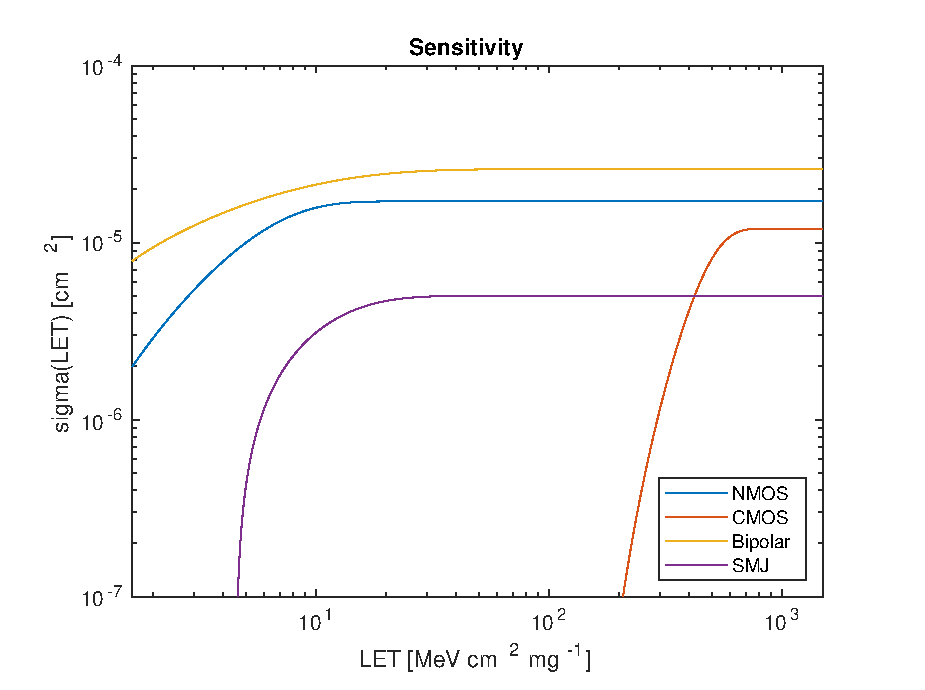
\includegraphics[width=.7\textwidth]{data/sigma/sensitivity.eps}
\caption{LET to sigma for multiple chips \ref{app:matlab:sigma}.}
\label{fig:matlab:LET-sigma-all}
\end{figure}

\begin{table}[H]
\centering
\begin{tabular}{|l|l|l|l|}
\hline
\textbf{Parameter} & \textbf{NMOS} & \textbf{CMOS} & \textbf{Bipolar} \\\hline

$L_0$ [MeV cm$^2$ mg$^{-1}$] & 0.487 & 136.8 & 0.6 \\\hline
$C_s$ [cm$^2$] & $1.71 \cdot 10^{-5}$ & $1.2 \cdot 10^{-5}$ & $2.6 \cdot 10^{-5}$ \\\hline
$W$   [MeV cm$^2$ mg$^{-1}$] & 4.95 & 350 & 4.4 \\\hline
$s$  ~ [arbitrary] & 1.422 & 3.0 & 0.7 \\\hline

\end{tabular}
\caption{NMOS2164, CMOS-R160-25 \& Bipolar 93L422 chip parameters.}
\label{tab:all-LET}
\end{table}



%----------------------------------------------------------------------------------------
%	SINGLE EVENT UPSETS ESTIMATION (Elrick).
%----------------------------------------------------------------------------------------
\subsection{\label{subsec:SEU-esti}Single Event Upsets Estimation}
The Single Event Upsets can be estimated using equation \ref{eq:LET2}, which is again shown below in equation \ref{eq:LET2-2}. The differential flux summed over the elements H (hydrogen) to U (uranium) $\sum^{92}_{Z=1} h(\text{LET})$ can be obtained from SPENVIS and can be seen in figure \ref{fig:LET-shielding}. The cross section based on the LET value is calculated in appendix \ref{app:matlab:sigma}. Calculating the total bit flips on average per day are shown in table \ref{tab:SEU-estimation}, together with the values that can be obtained from SPENVIS. It can be seen that the CMOS has the lowest amount of single event upsets and is thus the best choice.
\begin{equation}
\dv{U}{t} = 4 \pi \int^{\infty}_0 \sigma(\text{LET}, \theta, \phi) \cdot \sum^{92}_{Z=1} h(\text{LET}) d(\text{LET})\label{eq:LET2-2}
\end{equation}



\begin{table}[H]
\centering
\begin{tabular}{|l|l|l|}
\hline
Chip & SEU MATLAB & SEU SPENVIS \\
	 & [bits day$^{-1}$] & [bits$^{-1}$ day$^{-1}$] \\\hline
NMOS 2164		& 7.3806 & $2.9373 \cdot 10^{-2}$ \\\hline
CMOS R160-25	& $1.51 \cdot 10^{-2}$ & - \\\hline
Bipolar 93L422	& 10.988 & $1.9085$ \\\hline
SMJ329C50G		& 1.6646 & - \\\hline
\end{tabular}
\caption{Single event upsets per chip from MATLAB and SPENVIS.}
\label{tab:SEU-estimation}
\end{table}









%----------------------------------------------------------------------------------------
%	CONCLUSION (-).
%----------------------------------------------------------------------------------------
\newpage
%----------------------------------------------------------------------------------------
%	CONCLUSION.
%----------------------------------------------------------------------------------------

\section{\label{sec:conclusion}Conclusion}

The mission Willzyx I is a hyperbolic orbit around the Earth and then going into the direction of interstellar space. The eccentricity is greater than 1, which means the orbit is not bound to Earth. The mission duration is primary when coming close to Earth, which means the length is about 3 days.\\

This project was intended to confirm or refute the survivability of the proposed mission Willzyx I with certain purposed design features and requirements. In order to do this the trajectory of the spacecraft and its interaction with the environment is simulated with encounters in the expected regions it passes through. After running the necessary simulations using SPENVIS, it can be conclude that the proposed design is well suited for its intended mission with no major changes required.\\

The interactions of the spacecraft with the environment it would encounter was simulated in order to optimize some parameters, like the shielding of the solar arrays which was found to be optimal at 65$\mu m$ thick. The shielding of the memory was found to be more than enough to comply with the mission requirements. \\

In order to have the least amount of change to get single event upsets (SEU's), the CMOS chip has been chosen. This chip uses less energy then a TTL chip and has a higher noise margin. It is expected to have $1.51 \cdot 10^{-2}$\,bits/day, with a shielding of 0.37\,cm of aluminium. This means that the chance can be neglected.


%----------------------------------------------------------------------------------------
%	REFERENCES.
%----------------------------------------------------------------------------------------
\newpage				% Start at new page.
\addcontentsline{toc}{section}{References}
\printbibliography


%----------------------------------------------------------------------------------------
%	APPENDICES.
%----------------------------------------------------------------------------------------
\newpage				% Start at new page.
\begin{appendices}
    %------------------------------------------------------------------------------------
    %	APPENDIX: MATLAB LET.
    %------------------------------------------------------------------------------------
     \section{\label{app:matlab:LET}MATLAB: LET integral calculation}
    \lstinputlisting[style=Matlab-editor]{data/LET/LET.m}
    
    %------------------------------------------------------------------------------------
    %	APPENDIX: MATLAB Cross Section.
    %------------------------------------------------------------------------------------
	\newpage    
    \section{\label{app:matlab:sigma}MATLAB: Components characteristics \& SEU estimation}
    \lstinputlisting[style=Matlab-editor]{data/sigma/crossSection.m}

\end{appendices}


\end{document}
